\documentclass[../rapport_MVEX01-11-05]{subfiles}
\begin{document}

\section{Dolda Markovmodeller (HMM)}\label{sec:HMM}
För att kunna klassificera dynamiska gester räcker det inte att 
analysera bilder var för sig. Man behöver en modell som kan beskriva
karakteristiska beteenden för sekvenser av bilder.

En dold Markovmodell eller Hidden Markov model (HMM) är en utökning
av den klassiska Markovmodellen som gjorts för att skapa en
signalmodell som beskriver ett system utifrån dess utdata.
En vanlig Markovmodell består av ett antal tillstånd sammankopplade
med övergångssannolikheter (se figur~\ref{fig:hmm-ergodic}). Man kan alltså
röra sig i Markovprocessen genom att i varje tidssteg följa en av kanterna
ut från tillståndet, och valet av kant sker genom en stokastisk process.

\begin{figure}[tb]
  \centering
  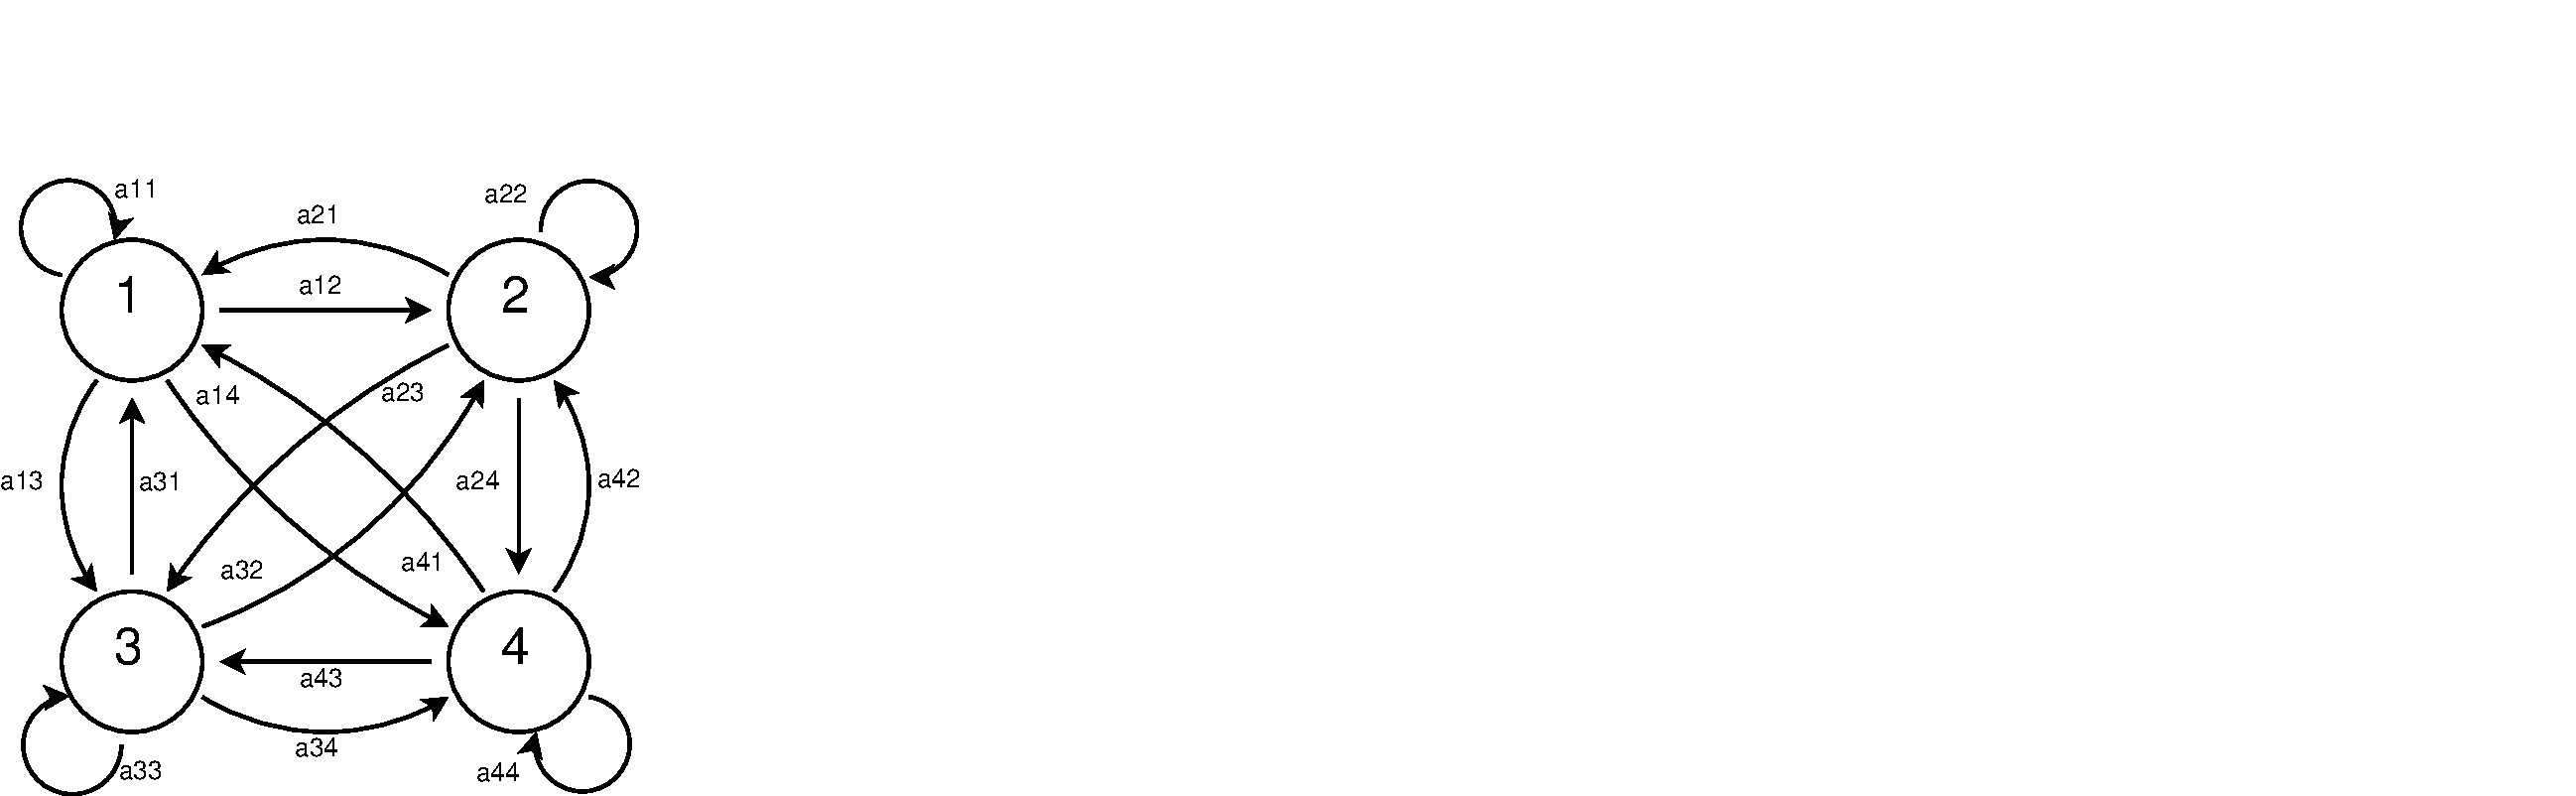
\includegraphics[width=0.8\textwidth,trim=0 0 935 80,clip=true]{bilder/ergodicHMM}
  \caption{En enkel, ergodisk Markovmodell med fyra tillstånd}
  \label{fig:hmm-ergodic}
\end{figure}

Det som är dolt i en HMM och som särställer den från en vanlig Markovmodell
är att varje tillstånd genererar
symboler efter ännu en sannolikhetsfördelning. Då man i vanliga Markovmodeller
observerar modellens tillstånd direkt, observeras nu istället de
symboler som genereras då tillstånden växlar. Dessa symboler motsvarar
den verkliga process man önskar modellera. Ett förtydligande exempel
är på sin plats: 

\begin{quote}
En person har ett antal tärningar --- vissa är viktade och avviker därmed
från den annars uniforma sannolikhetsfördelningen.
Han kastar en tärning ur sin
samling och berättar för en kompis hur många ögon tärningen
visar. Därefter avgör tärningskastaren om han vill byta tärning eller
inte, och upprepar proceduren. Kompisen får alltså inte se vilken av
tärningarna som kastas för tillfället, utan får bara ta del av vad
respektive tärning visar. Denna process skulle kunna beskrivas med
hjälp av en HMM där varje enskild tärning representerar ett
tillstånd, och antalet ögon som visas är en symbol.
Den förstnämnda personen rör sig mellan tärningarna
(tillstånden) efter eget behag och tillkännager enbart värdet
(symbolerna) som genereras av dem. 
\end{quote}

För att tillämpa detta vi gestigenkänning måste man konstruera en HMM
för varje gest som finns med i systemet. Klassificeringen görs sedan genom
att välja den HMM som bäst beskriver den observerade datan. Symbolerna
tilldelas exempelvis genom någon typ av enklare klassificering av bilddata
som resulterar i ett mindre antal ''typbilder''. Tillstånden motsvarar
då i någon mening olika skeden av gesterna.

% (Kan även nämna Starner98, Rigol98)}

\subsection{Beståndsdelarna av en HMM}
En HMM karakteriseras av följande beståndsdelar:
\begin{itemize}
\item $N$, antalet tillstånd i modellen. Vi betecknar de olika
  tillstånden som $S = \{S_1, S_2, \dots, S_N\}$, och tillståndet vid
  tiden $t$ som $q_t$.
\item $M$, antalet distinkta observationssymboler för ett givet
  tillstånd. De individuella symbolerna betecknar vi som $V =
  \{v_1,v_2,\dots,v_M\}$.
\item $A$,en övergångsmatris där varje element ger sannolikheten att
  vandra från ett tillstånd till ett annat, 
\begin{equation*}
a_{ij} = \Prob(q_{t+1} = S_j|q_t = S_i),\quad 1 \leq i,j \leq N.
\end{equation*}
I fallet då man kan nå alla tillstånd från vilket tillstånd som helst
med ett enda steg har vi alltså $a_{ij} > 0,\;\forall i,j$. 
\item $b_j(k)$, sannolikhetsfördelningar för observationssymboler givet ett
  specifikt tillstånd $j$, där 
\begin{equation*}
b_j(k) = \Prob(v_k \text{ vid tiden } t|q_t = S_j) \quad 1 \leq j \leq N,\quad1 \leq k \leq M.
\end{equation*}
$b_j(k)$ ger med andra ord sannolikheten att symbolen $v_k$ genereras
då vi befinner oss i tillstånd $j$.
\item Sannolikhetsfördelningen för ett begynnelsetillstånd, $\pi =
  \{\pi_i\}$, där
\begin{equation*}
\pi_i = \Prob(q_1 = S_i).
\end{equation*}
\end{itemize}
Givet parametrarna $M$ och $N$, en specificering av symboler, samt de
tre sannolikhetsmåtten $A, B$ och $\pi$ är det möjligt att
fullständigt specificera en HMM. I fortsättningen kommer vi att
använda oss av den kompaktare notationen $\lambda = (A,B,\pi)$
för att representera parametrarna för en given HMM.

\subsection{Grundläggande problem}
För att kunna föra över modellen från teori till praktisk tillämpning
återstår flera viktiga detaljer. \citeasnoun{Rabiner89} presenterar
tre grundläggande frågor för implementeringen av en HMM, varav följande
två är av intresse i den här rapporten:
\begin{description}
\item[Problem 1:] Givet en sekvens av observationer
  $\vect{O}=\{O_1,O_2,\dots,O_t\}$ och en modell $\lambda = (A,B,\pi)$, hur
  beräknar man $\Prob(\vect{O}|\lambda)$? Dvs. vad är sannolikheten att
  sekvensen genererades av modellen $\lambda$? Hur kan
  det göras så effektivt som möjligt? Effektivitetsfrågan visar sig
  vara ytterst viktig. 
\item[Problem 2:] Hur går man tillväga för att optimera
  $\Prob(\vect{O}|\lambda)$ genom att justera
  modellparametrarna $\lambda = (A,B,\lambda)$? 
\end{description}

Kan man lösa det första problemet har man möjlighet att uppskatta hur
väl en modell matchar en viss observationsföljd. Man kan se det som
ett sätt att jämföra olika modeller och
deras relation till en specifik observationsföljd. Denna synvinkel är
mycket användbar då man ställs inför utmaningen att välja mellan
flera existerande modeller. 

Det andra problemet behandlar modelloptimering. Hur kan på bästa
sätt anpassa en modell till en viss observationsföljd?
Lösningen till detta problem utgör en fundamental del av
att skapa modellen i  praktiken.
Med hjälp av en träningssekvens, alltså en följd av
observationer, kan man då träna en HMM. Vikten av att
optimeringsprocessen ger bra resultat är stor eftersom
träningssekvensen utgör den enda kopplingen till det verkliga fenomen
man önskar modellera.      

\subsection{Framåt-bakåt-tekniken}
En användbar teknik för att lösa det första problemet introducerades av \citeasnoun{Baum67}, kallad
\emph{forward-backward}-proceduren. Vi
definierar framåtvariabeln $\alpha_t(i)$ enligt
\begin{equation*}
\alpha_t(i) = \Prob(O_1,O_2,\dots,O_t,q_t = S_i | \lambda),
\end{equation*}
alltså sannolikheten att ha genererat observationsföljden $\textbf{O}
= \{O_1,O_2,\dots,O_t$\} samt befinna sig i tillstånd $S_i$ vid tiden
$t$, givet en modell $\lambda$. En av metodens fördelar är att man med
hjälp av induktion kan finna $\alpha_t(i)$ genom följande process:

\begin{enumerate}
\item Initialisering:
\begin{equation*}
\alpha_1(i) = \pi_ib_i(O_1), \quad 1\leq i \leq N
\end{equation*}

\item Induktion:
\begin{equation*}
\alpha_{t+1}(j) =
\left(\sum_{i=1}^N\alpha_t(i)a_{ij}\right)b_j(O_{t+1}) \quad 1 \leq t \leq T-1,\quad1 \leq j \leq N
\end{equation*}

\item Avslutning:
\begin{equation*}
\Prob(\vect{O}|\lambda) = \sum_{i=1}^N\alpha_T(i)
\end{equation*}
\end{enumerate}

I första steget, då $t=1$, initialiseras framåtvariabeln $\alpha_1(i)$ som
sannolikheten att börja i tillstånd $S_i$ och därefter generera
observation $O_1$. För $t=2$ använder man sedan induktionssteget. Utgår man
från första steget kan man övertyga sig om att
$\sum_{i=1}^N\alpha_1(i)a_{ij}$ måste vara den totala sannolikheten
att hamna i $S_j$ vid $t=2$, efter att ha genererat $O_1$ i föregående
tillstånd.

Efter multiplikation med $B_j(O_{2})$ fås därefter
sannolikheten att generera $O_2$, då man befinner sig i $S_j$ med en
observerad symbol $O_1$, eller med andra ord, $\Prob(O_1,O_2,S_j
= q_2 | \lambda) = \alpha_2(j)$. Fortsätter man på samma vis har man
slutligen $\alpha_T(i) = \Prob(O_1,O_2,\dots,O_T,S_i = q_T |
\lambda)$.

Sista steget ger slutligen svaret på vårt första problem, nämligen
sannolikheten $\Prob(\vect{O}|\lambda)$. Detta inses lätt då vi
använder oss av definitionen av $\alpha_T(i)$, 
\begin{equation*}
\Prob(\vect{O}|\lambda) = \sum_{i=1}^N\alpha_T(i) =
\sum_{i=1}^N\Prob(O_1,O_2,\dots,O_T,q_T = S_i|\lambda). 
\end{equation*} 

Med andra ord är sannolikheten att generera observationsföljden
$\vect{O}$ summan av sannolikheterna att generera $\vect{O}$ med
sluttillstånd $S_i$, $1 \leq i \leq N$.

\subsection{Iterativ metod för träning av HMM}
Med en lösning till första problemet i bagaget kan man tackla nästa,
själva träningen av en HMM. Detta är ett betydligt mer invecklat
problem än det tidigare, med betydligt fler angreppsvinklar. En
analytisk lösning till optimeringsproblemet är inte känd, utan man
tvingas istället använda sig av Baum-Welch-metoden eller
gradient-tekniker \cite{Dempster77,Levinson83}. 
Givet en ändlig observationssekvens går det inte att optimera modellens parametrar globalt \cite{Rabiner89}.
Däremot kan man välja $\lambda = (A,B,\pi)$ på så sätt att $\Prob(\vect{O}|\lambda)$ är lokalt
maximerad. 

Baum-Welch-metoden utgår från bakåtvariabeln $\beta_t(i)$ som likt
framåtvariabeln $\alpha_t(i)$ definieras enligt
\begin{equation*}
\beta_t(i) = \Prob(O_{t+1},O_{t+2},\dots,O_T | q_t = S_i, \lambda).
\end{equation*} 

$\beta_t(i)$ är alltså sannolikheten att observera en delsekvens av
observationer då man startar i tillstånd $S_i$. Processen för att beräkna $\beta_t(i)$ består av två steg:
\begin{enumerate}
\item Initialisering: 
\begin{equation*}
\beta_T(i) = 1, \quad 1 \leq i \leq N.
\end{equation*}
\item Induktion: 
\begin{equation*}
\beta_t(i) = \sum\limits_{j=1}^Na_{ij}b_j(O_{t+1})\beta_{t+1}(j), \quad t =
T-1,T-2,\dots,1 \quad 1 \leq i \leq N.
\end{equation*}
\end{enumerate}

Inledningsvis sätts $\beta_T(i)$ godtyckligt till 1, varefter
induktionssteget fungerar efter samma princip som för framåtvariabeln
$\alpha$.

Framåt- och bakåtvariablerna kan användas tillsammans
för att bilda två nya variabler $\xi_t$ och $\gamma_t$.
Den första definieras som 
\begin{equation*}
\xi_t(i,j) = P(q_t = S_i, q_{t+1} = S_j|\vect{O},\lambda),
\end{equation*}
alltså sannolikheten att befinna sig i tillstånd $S_i$ och
därefter i $S_j$. Genom $\alpha$ och $\beta$ kan den uttryckas som
\begin{equation*}
\xi_t(i,j) = \frac{\alpha_t(i)a_{ij}b_j(O_{t+1})\beta_{t+1}(j)}{\Prob(\vect{O}|\lambda)}
\end{equation*} 
där $\Prob(\vect{O}|\lambda)$ normerar $\xi_t$ så att den blir ett korrekt
sannolikhetsmått.

Den andra variabeln, som beskriver hur många gånger tillståndet $S_i$ besöks
vid tiden $t$, kan uttryckas
\begin{equation*}
\gamma_t(i) = \sum_{j=1}^N\xi_t(i,j).
\end{equation*}

Summerar vi sedan $\gamma_t(i)$ över tiden $t$ får vi en storhet
som kan tolkas som antalet gånger tillståndet $S_i$ har besökts,
eller antalet förflyttningar från tillståndet $S_i$:
\begin{equation*}
\sum_{t=1}^{T-1}\gamma_t(i) = \text{antalet förväntade förflyttningar
  från tillstånd $S_i$.}
\end{equation*} 

På samma sätt kan summation över tiden hos  $\xi_t(i,j)$ förklaras:
\begin{equation*}
\sum_{t=1}^{T-1}\xi_t(i,j) = \text{antalet förväntade förflyttningar
  från tillstånd $S_i$ till $S_j$}.
\end{equation*}

Notera att efterson $\xi_t(i,j)$ inte är definierad för $t=T$ går summationen 
endast upp till $T -1$. 

Den iterativa metoden som återuppskattar modellens parametrar $A,B$
och $\pi$ kan nu skrivas som
\begin{equation*}
\bar{\pi} = \text{[förväntat antal gånger i tillstånd $S_i$ vid
  $t=1$]} = \gamma_i(i),
\end{equation*}
\begin{multline*}
\bar{a}_{ij} = \\ = \frac{\text{förväntat antal förflyttningar från
    tillstånd $S_i$ till $S_j$}}{\text{förväntat antal förflyttningar
    från tillstånd $S_i$}} = \\ =
\frac{\sum_{t=1}^{T-1}\xi_t(i,j)}{\sum_{t=1}^{T-1}\gamma_t(i)},
\end{multline*}
\begin{multline*}
\bar{b}_j(k) = \\ = \frac{\text{förväntat antal gånger i tillstånd $S_j$
    och observerandes symbol $v_k$}}{\text{förväntat antal gånger i
    tillstånd $S_j$}} = \\ = \frac{\sum_{\substack{t=1\\s.t~ O_t =
      v_k}}^{T-1}\gamma_t{j}}{\sum_{t=1}^{T-1}\gamma_t(j)}.
\end{multline*}

Vänsterleden fås genom att ta den nuvarande modellen $\lambda =
(A,B,\pi)$, sedan beräkna högerleden, och därigenom erhålla $\bar{\lambda} =
(\bar{A},\bar{B}, \bar{\pi})$. \citeasnoun{Baum68} och \citeasnoun{Baker75}
visade att denna iterativa process resulterar antingen i
\begin{inparaenum}[\itshape1\upshape)]
	\item ett lokalt maximum för $\Prob(\vect{O}|\lambda)$
  (alltså att $\lambda = \bar{\lambda}$), eller
 	\item i en förbättrad modell $\bar{\lambda}$ på så sätt att
  $\Prob(\vect{O}|\bar{\lambda}) > \Prob(\vect{O}|\lambda)$
\end{inparaenum}. 

\subsection{Olika typer av HMM}
Då man talar om olika typer av HMM syftar man först och främst på
typen av övergångsmatris som används. Hittills har bara 
fallet där $a_{ij} > 0$ för alla $i,j$ nämnts --- detta kallas en ergodisk
modell. Detta innebär att varje tillstånd i modellen
kan nås från alla andra tillstånd inom ändlig tid. Om man
tänker sig en modell med fyra tillstånd får man följaktligen övergångsmatrisen
\begin{equation*}
A = \begin{bmatrix}
a_{11} & a_{12} & a_{13} & a_{14}\\
a_{21} & a_{22} & a_{23} & a_{24}\\
a_{31} & a_{32} & a_{33} & a_{34}\\
a_{41} & a_{42} & a_{43} & a_{44}
\end{bmatrix}.  
\end{equation*} 

Det har dock visats att andra typer av modeller i vissa fall presterar
bättre än den ergodiska. \citeasnoun{Elmezain08}
presenterar resultat som pekar ut Bakis-modellen, även kallad
vänster-höger-modellen, som den främsta då det gäller modellering
av tidsvarierande signaler. Bakis-modellen fungerar på så sätt att den
inte tillåter förflyttning till ett ''tidigare'' tillstånd. Elementen i
övergångsmatrisen A tvingas med andra ord efterfölja restriktionen
\begin{equation*}
a_{ij} = 0 \quad\text{om }j<i,
\end{equation*}
och matrisen blir uppåt triangulär.
Vidare får sannolikhetsfördelningen för begynnelsetillstånd följande
utseende
\begin{equation*}
\pi_i = \begin{cases}
         1 & \quad\text{om } i = 1\\
         0 & \quad\text{om } i \neq 1.\end{cases}.
\end{equation*}  

\begin{figure}[tb]
  \centering
  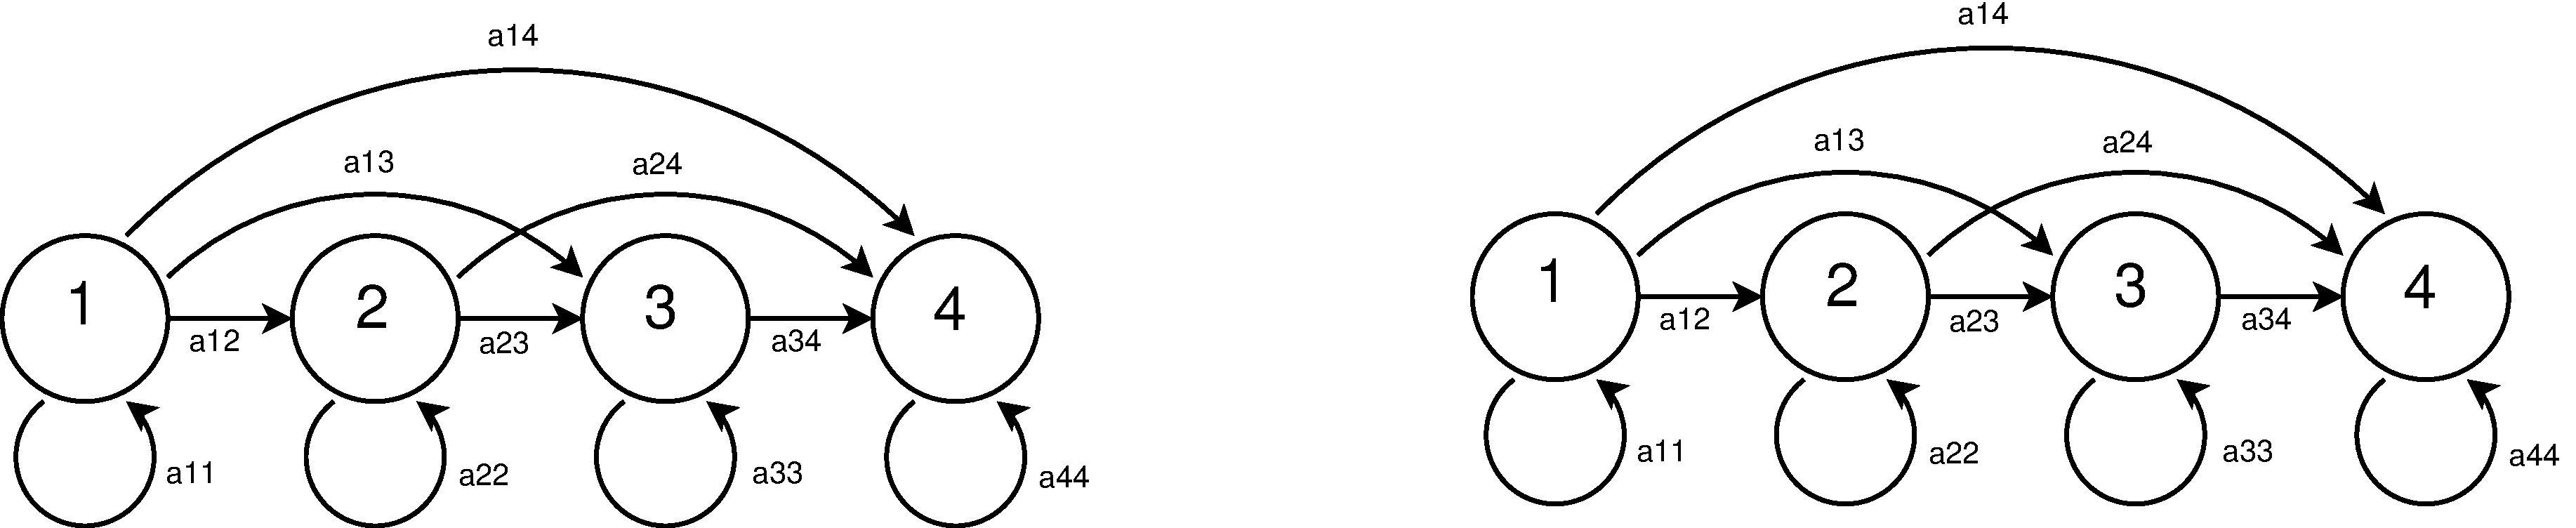
\includegraphics[width=0.8\textwidth,trim=0 0 1010 10,clip=true]{bilder/LR_HMM}
  \caption{En Markovmodell av Bakis-modellen med fyra tillstånd}
  \label{fig:hmm-lr}
\end{figure}

Man startar alltså alltid i det första tillståndet för att sedan
stanna kvar i samma tillstånd eller röra sig åt höger (se
figur~\ref{fig:hmm-lr}). Antalet steg
man tar är inte begränsat på annat sätt än att det slutgiltiga
tillståndet $S_N$ inte får passeras. Denna modell användes av
\citeasnoun{Yamato92} och skiljer sig i vissa avseenden från
den som den som används av \citeasnoun{Elmezain08}, t.ex.~på det sätt att
den bara tillåter förflyttning från
ett tillstånd till sig självt eller till nästa (man får alltså inte ''hoppa
över'' tillstånd, se figur~\ref{fig:hmm-lrb}), ett val som ger upphov
till övergångsmatrisen
\begin{equation*}
A = \begin{bmatrix}
a_{11} & a_{12} & 0 & 0\\
0 & a_{22} & a_{23} & 0\\
0 & 0 & a_{33} & a_{34}\\
0 & 0 & 0 & a_{44}
\end{bmatrix}.  
\end{equation*} 

\begin{figure}[tb]
  \centering
  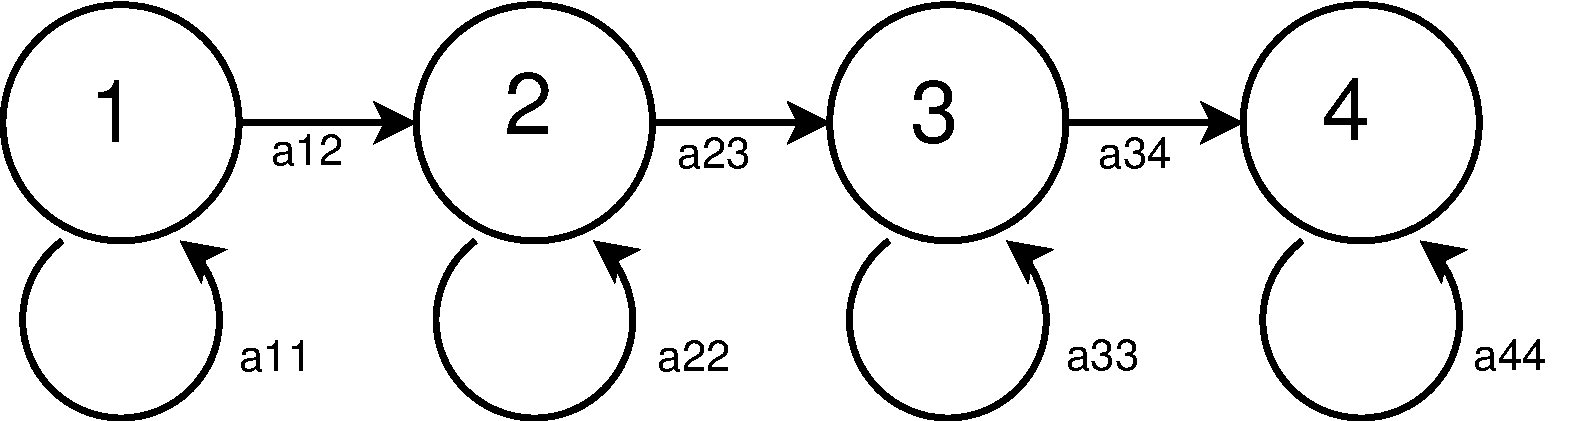
\includegraphics[width=0.8\textwidth]{bilder/LRB_HMM}
  \caption{En Markovmodell med fyra tillstånd enligt
  \protect\possessivecite{Yamato92} modell}
  \label{fig:hmm-lrb}
\end{figure}

Utöver dessa varianter finns det självklart otaliga andra då man kan
sammanbinda de olika tillstånden helt efter eget tycke.

\end{document}
